\documentclass{report}
\usepackage[utf8]{inputenc}
\usepackage{natbib}
\usepackage{graphicx}
\usepackage[pagestyles]{titlesec}

\title{Design Document}
\author{AmorosiniCasaliFioravanti}
\date{December 2019}

\titleformat{\chapter}[display]{\normalfont\bfseries}{}{0pt}{\Huge}
\newpagestyle{mystyle}
{\sethead[\thepage][][\chaptertitle]{}{}{\thepage}}
\pagestyle{mystyle}

\begin{document}

\maketitle

\chapter{Introduction}
While the RASD presented a general view of the SafeStreets appliction and its features, this document aims to further analyze the system's design and architecture, by describing for each of its components their runtime behaviour, integration, interfaces, implementation and testing plans.
This document is mainly intended to be used by the test and development teams as a guidance in the development process, but also to prevent structural degradation during maintainance and extension phases. Nonetheless, the document is also addressed to all the stakeholders who are interested in supervising the development process.

\section{Purpose}
%Frase generata automaticamente da overleaf ma non per questo meno vera:
``I always thought something was fundamentally wrong with the universe'' 

\section{Scope}

\chapter{Architectural Design}
\section{Overview}
In this chapter we are going to discuss the architectural structure of the System. In Figure 1 is represented an high-level view of the components and their interactions. The details are explained in the next sections.
\begin{figure}[!ht]
	\begin{center}
	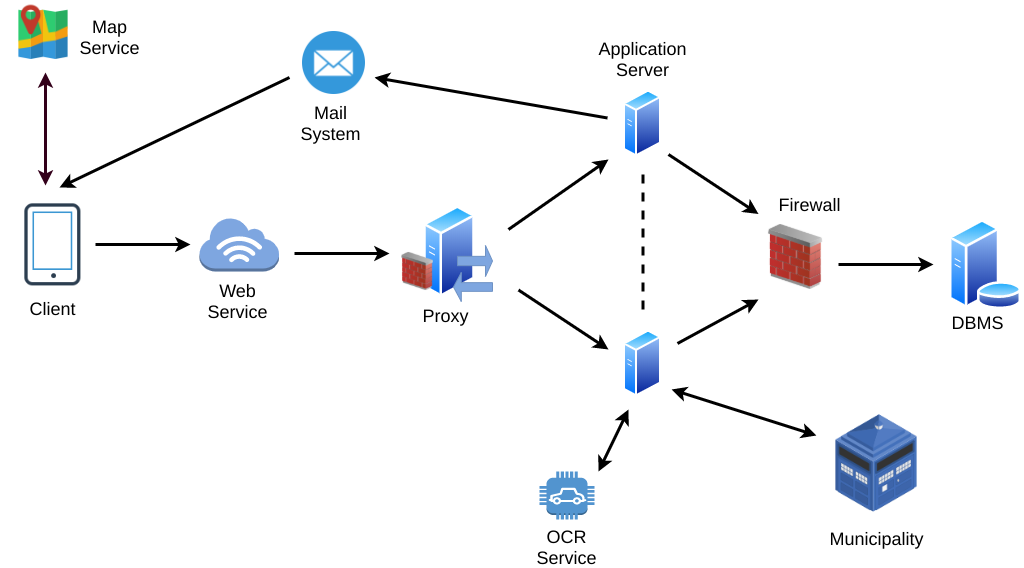
\includegraphics[width=\textwidth]{img/HighLevelOverview.png}
	\end{center}
	\caption{Overview of the System.}
\end{figure}

\section{Component view}

\section{Deployment view}

\section{Runtime view}

\section{Component interfaces}

\section{Selected architectural	styles and patterns}
The following architecture are used for the structure of the System.
\subsection{Client-Server Architecture}
In this structure there are two main role with different duties, the client uses data and services offered by the server.
 The server stores all data in order to provide them to the client.\\
\textbf{Motivations:} this pattern dues to several advantages. Server can be replicated to have more scalability. 
Accessibility: users can use the services without the need for a specialized​ ​device​ ​or​ ​client.
The security is granted because the server allows only registered user to consult data.
Furthermore, it is easy to update, replace, repair, move a server without affecting clients.
\subsection{Three-tiered Architecture}
This type of architecture is a client-server architecture where three tiers are phisically separated.\\
The \textit{presentation tier} provide an interface to allow the user to consult data and result of services executed in a different layer. 
It is the top-most tier and the only one accessible from the client.\\
The \textit{application tier} executes the logic of the application throw functions that elaborate data. 
The reverse proxy is needed to handle the client requests and to balance the workload, the requests are forwarded to 
the application serves in order to provide the right data.\\
The \textit{database tier} includes the data persistence mechanisms and the data access layer that encapsulates 
the persistence mechanisms and exposes the data.
\begin{figure}[!ht]
	\begin{center}
	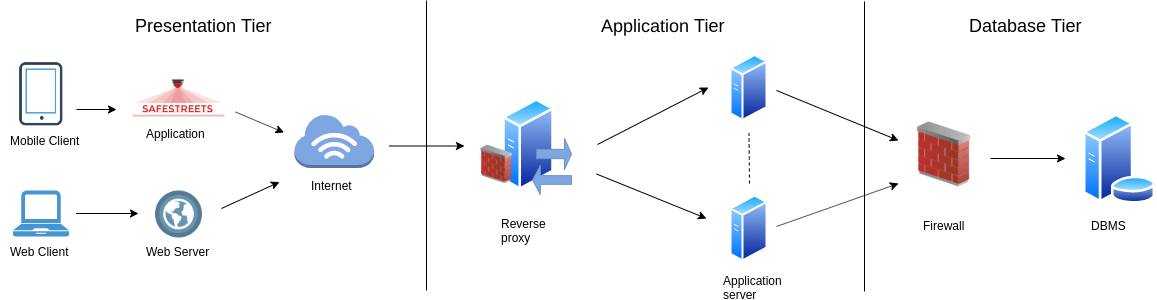
\includegraphics[width=\textwidth]{img/TiersArchitecture.png}
	\end{center}
	\caption{Overview of the System.}
\end{figure}

\end{document}